\subsection{Sistema de Medición}

Con lo tratado en la sección del sistema de control del capítulo \ref{analisis}, se estableció que para realizar un adecuado control de la plataforma, se debe tomar información de cuatro variables de estado del sistema: la tensión y corriente de la pila de combustible ($v_{FC}$ e $i_{FC}$) y la tensión y corriente de salida ($v_o$ e $i_o$). En esta sección se va a tratar el diseño del sistema de medición de datos de la figura \ref{diag_medicion}, que incluye el sensado de los parámetros del convertidor, el acondicionamiento de las señales, y la transmisión de las mismas al sistema de control.\\

\begin{figure}[h]
    \centering
    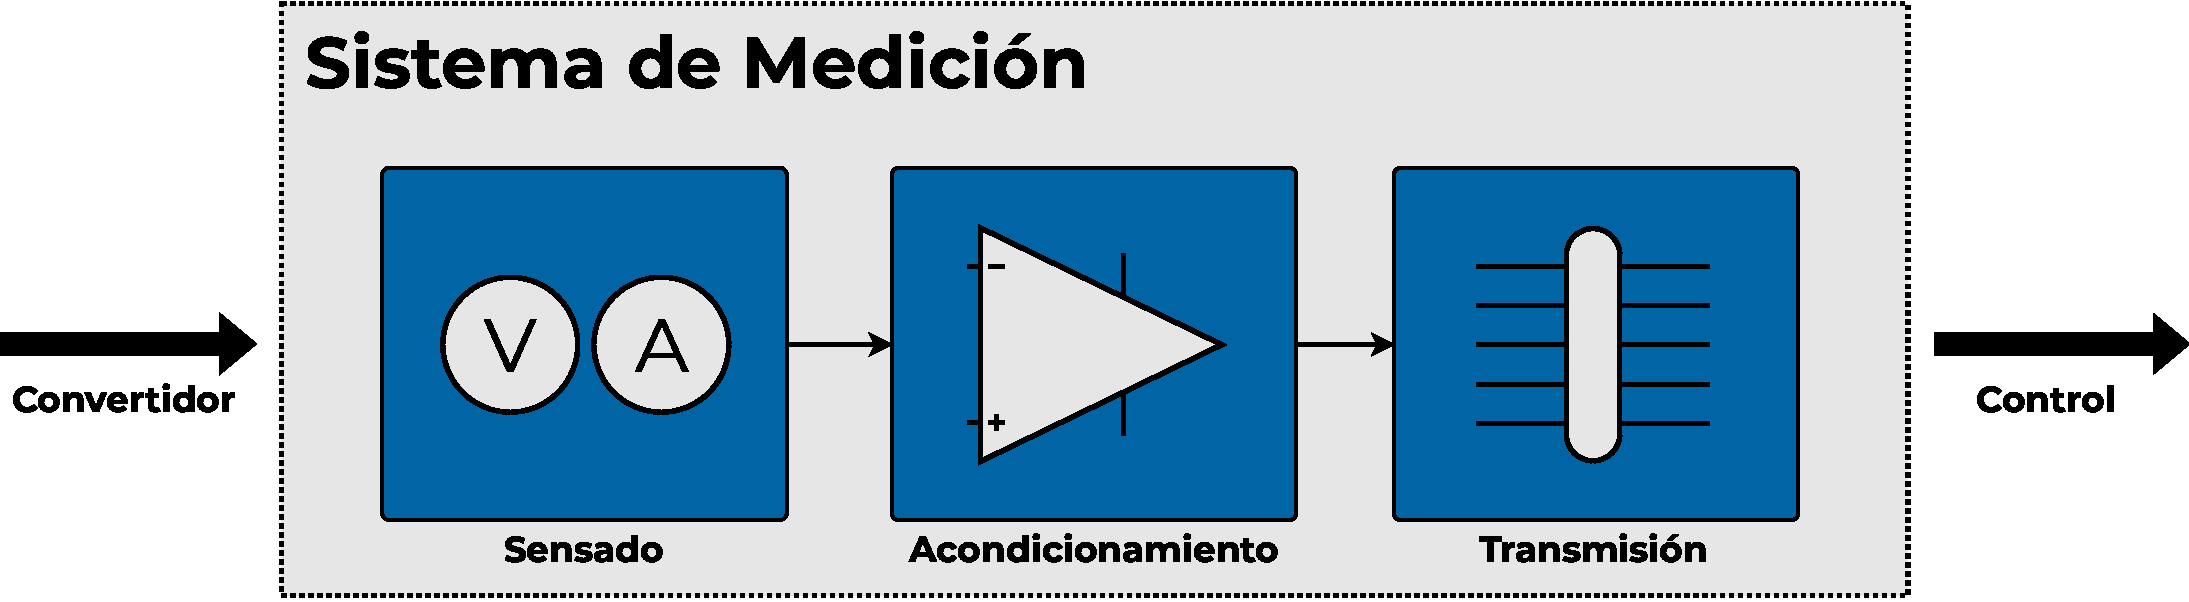
\includegraphics[scale=0.4]{Imagenes/Sistema Medicion.pdf}
    \caption{Sistema de medición de la plataforma, con las tres etapas que lo conforman.}
    \label{diag_medicion}
\end{figure}

Este sistema comienza con la adquisición de los parámetros de interés provenientes del convertidor, tarea llevada a cabo por los sensores de tensión y corriente que conforman la {\Medium etapa de sensado}. Sin embargo, estos datos obtenidos no se presentan en una forma que nuestro sistema de control sea capaz de procesar, por lo que se necesita la siguiente etapa del sistema, la {\Medium etapa de acondicionamiento}, que se encarga de adecuar los datos obtenidos por los sensores para que puedan ser utilizados por el controlador. Finalmente, necesitamos una forma de llevar estos datos desde el sistema de medición hasta el controlador, función que es llevada a cabo por el último bloque de la figura, la {\Medium etapa de transmisión}.\\

Vamos a tratar el diseño de este sistema en el orden que se observa en la figura, por lo que se comenzará por la etapa de sensado o adquisición de datos.\\

\subsubsection{Etapa de Sensado}

En este sistema, los únicos parámetros a medir son tensiones y corrientes, tanto de la pila de combustible a la entrada como de la carga variable a la salida. Previamente a la seleccion de los sensores a utilizar, vamos a realizar una breve categorización y explicación de los métodos de sensado disponibles para ambos parámetros, comenzando por las tensiones.\\

\paragraph{Tecnologías de Sensado de Tensión}

Este es el más simple de los dos casos, ya que los sistemas de control ya trabajan con señales expresadas en tensiones, por lo que no es requerido ningún tipo de transductor, únicamente una adaptación de niveles que es llevada a cabo por la etapa de acondicionamiento. Por esta razón, lo único necesario en este caso es la obtención directa de la tensión buscada, siempre minimizando la perturbación que esta medición introduce al sistema.\\

\paragraph{Tecnologías de Sensado de Corriente}

A diferencia del caso de las tensiones, para poder obtener una medición de corriente se debe realizar algún tipo de transducción que transforme la información de corriente en valores de tensión que puedan ser utilizados por el sistema de control. Existen múltiples tecnologías de sensado y transucción de corriente fundamentalmente distintas, cada una con sus propias características, ventajas y desventajas. Vamos a dedicar algunos párrafos a su clasificación y descripción.\\

\subparagraph{Resistencia Shunt}

Es el método conceptualmente más sencillo de todos, y consiste en interponer al camino de la corriente un resistor \textit{shunt} $R_S$, es decir una resistencia de muy bajo valor (generalmente en las decenas y unidades de \unit{\milli\ohm}), y luego medir la caída de tensión en el mismo. Esta corriente se encuentra directamente relacionada con la tensión mediante la Ley de Ohm, que luego de reordenar resulta:

\begin{equation*}
    I=\frac{1}{R_S}V_S
\end{equation*}

Entonces, con este método se obtiene una relación {\Medium perfectamente lineal} entre entre la tensión medida directamente y la corriente que se quiere obtener, siendo el inverso del valor del resistor (o su conductancia) la constante de proporcionalidad. Al tener la Ley de Ohm como su principio de funcionamiento, este método es capaz de medir todo tipo de corrientes, tanto continua (CC) como alterna (CA). Además, al necesitar únicamente una resistor, es {\Medium sumamente sencillo} de implementar.\\

Sin embargo, al estar circulando toda la corriente a través del resistor, se genera una {\Medium pérdida de energía significativa}, ya que la potencia disipada depende del cuadrado de la corriente. Si tomamos la plataforma como ejemplo, donde la corriente de pila $i_{FC}$ en el primario puede llegar a un máximo de \SI[]{10}[]{\ampere}, una resistencia shunt de \SI[]{50}[]{\milli\ohm} puede llegar a disipar una potencia de \SI[]{5}[]{\watt}. Por esta razón, este método no es factible para mediciones de grandes corrientes.\\

La precisión de este método también se {\Medium deteriora con la frecuencia}, ya que para frecuencias suficientemente altas, los efectos de la inductancia parásita $L_S$ y el efecto skin generan un aumento de la impedancia que afecta a la medición.\\

Dadas las altas potencias que puede llegar a disipar un resistor shunt, la temperatura puede presentar un problema si su coeficiente de temperatura no es adecuado. Los fabricantes de estas resistencias tienen esto en cuenta y fabrican los componentes con materiales de bajo coeficiente de temperatura.\\

\begin{figure}[h]
    \centering
    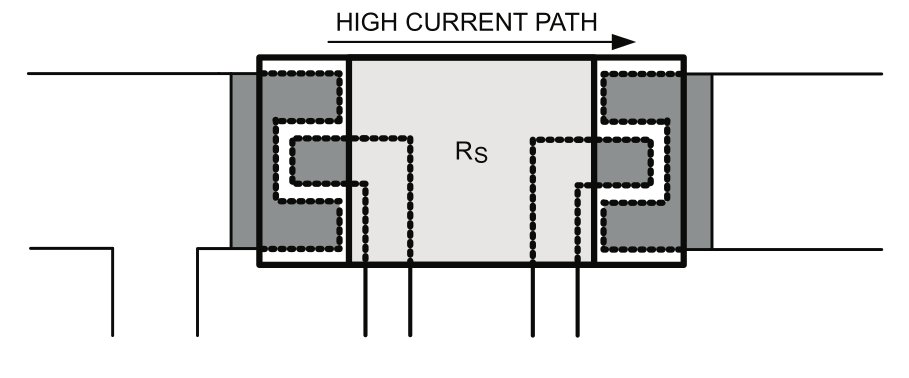
\includegraphics[scale=1]{Imagenes/Conexion Kelvin.png}
    \caption{Conexión Kelvin de cuatro cables para el sensado de corriente con un resistor shunt.}
    \label{conexion_kelvin}
\end{figure}

Sin embargo, esto no puede solucionar el error introducido por el coeficiente de temperatura de las soldaduras, que se exacerban particularmente para valores bajos de resistencia. Para solventarlo, se debe utilizar la conexión de cuatro cables o Kelvin, que separa el camino de alta corriente de las conexiones de sensado, como se ve en la figura \ref{conexion_kelvin}.\textsuperscript{\cite{CurrentSensing}}\\

\subparagraph{Transformador de Corriente}

\lipsum[2]\\

\subparagraph{Bobina de Rogowski}

\lipsum[3]\\

\subparagraph{Efecto Hall}

\lipsum[4]\\

\subsubsection{Etapa de Acondicionamiento}

\lipsum[1]\\

\subsubsection{Etapa de Transmisión}

\lipsum[2]\\

\lipsum[3]\\